% Created by tikzDevice version 0.12.4 on 2023-11-09 11:30:43
% !TEX encoding = UTF-8 Unicode
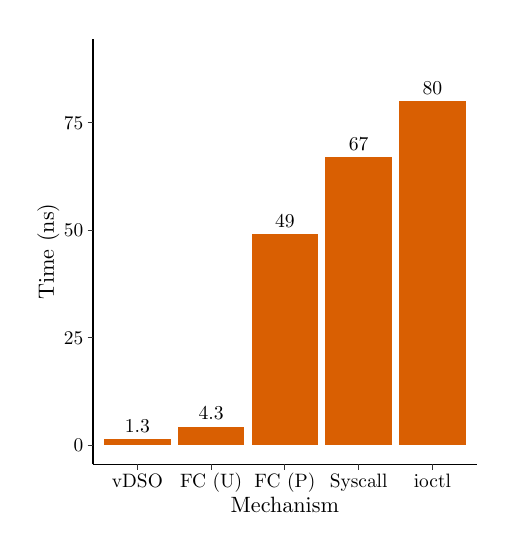
\begin{tikzpicture}[x=1pt,y=1pt]
\definecolor{fillColor}{RGB}{255,255,255}
\path[use as bounding box,fill=fillColor,fill opacity=0.00] (0,0) rectangle (166.22,180.67);
\begin{scope}
\path[clip] (  0.00,  0.00) rectangle (166.22,180.67);
\definecolor{drawColor}{RGB}{255,255,255}
\definecolor{fillColor}{RGB}{255,255,255}

\path[draw=drawColor,line width= 0.4pt,line join=round,line cap=round,fill=fillColor] (  0.00,  0.00) rectangle (166.22,180.68);
\end{scope}
\begin{scope}
\path[clip] ( 23.66, 22.85) rectangle (162.22,176.67);
\definecolor{fillColor}{RGB}{255,255,255}

\path[fill=fillColor] ( 23.66, 22.85) rectangle (162.22,176.67);
\definecolor{fillColor}{RGB}{217,95,2}

\path[fill=fillColor] (134.24, 29.84) rectangle (158.22,154.14);

\path[fill=fillColor] (107.60, 29.84) rectangle (131.58,133.94);

\path[fill=fillColor] ( 80.95, 29.84) rectangle (104.93,105.98);

\path[fill=fillColor] ( 27.66, 29.84) rectangle ( 51.64, 31.86);

\path[fill=fillColor] ( 54.31, 29.84) rectangle ( 78.29, 36.52);
\definecolor{drawColor}{RGB}{0,0,0}

\node[text=drawColor,anchor=base,inner sep=0pt, outer sep=0pt, scale=  0.71] at (146.23,156.59) {80};

\node[text=drawColor,anchor=base,inner sep=0pt, outer sep=0pt, scale=  0.71] at (119.59,136.39) {67};

\node[text=drawColor,anchor=base,inner sep=0pt, outer sep=0pt, scale=  0.71] at ( 92.94,108.43) {49};

\node[text=drawColor,anchor=base,inner sep=0pt, outer sep=0pt, scale=  0.71] at ( 39.65, 34.31) {1.3};

\node[text=drawColor,anchor=base,inner sep=0pt, outer sep=0pt, scale=  0.71] at ( 66.30, 38.97) {4.3};
\end{scope}
\begin{scope}
\path[clip] (  0.00,  0.00) rectangle (166.22,180.67);
\definecolor{drawColor}{RGB}{0,0,0}

\path[draw=drawColor,line width= 0.6pt,line join=round] ( 23.66, 22.85) --
	( 23.66,176.67);
\end{scope}
\begin{scope}
\path[clip] (  0.00,  0.00) rectangle (166.22,180.67);
\definecolor{drawColor}{RGB}{0,0,0}

\node[text=drawColor,anchor=base east,inner sep=0pt, outer sep=0pt, scale=  0.70] at ( 20.06, 27.43) {0};

\node[text=drawColor,anchor=base east,inner sep=0pt, outer sep=0pt, scale=  0.70] at ( 20.06, 66.27) {25};

\node[text=drawColor,anchor=base east,inner sep=0pt, outer sep=0pt, scale=  0.70] at ( 20.06,105.12) {50};

\node[text=drawColor,anchor=base east,inner sep=0pt, outer sep=0pt, scale=  0.70] at ( 20.06,143.96) {75};
\end{scope}
\begin{scope}
\path[clip] (  0.00,  0.00) rectangle (166.22,180.67);
\definecolor{drawColor}{gray}{0.20}

\path[draw=drawColor,line width= 0.4pt,line join=round] ( 21.66, 29.84) --
	( 23.66, 29.84);

\path[draw=drawColor,line width= 0.4pt,line join=round] ( 21.66, 68.68) --
	( 23.66, 68.68);

\path[draw=drawColor,line width= 0.4pt,line join=round] ( 21.66,107.53) --
	( 23.66,107.53);

\path[draw=drawColor,line width= 0.4pt,line join=round] ( 21.66,146.38) --
	( 23.66,146.38);
\end{scope}
\begin{scope}
\path[clip] (  0.00,  0.00) rectangle (166.22,180.67);
\definecolor{drawColor}{RGB}{0,0,0}

\path[draw=drawColor,line width= 0.6pt,line join=round] ( 23.66, 22.85) --
	(162.22, 22.85);
\end{scope}
\begin{scope}
\path[clip] (  0.00,  0.00) rectangle (166.22,180.67);
\definecolor{drawColor}{gray}{0.20}

\path[draw=drawColor,line width= 0.4pt,line join=round] ( 39.65, 20.85) --
	( 39.65, 22.85);

\path[draw=drawColor,line width= 0.4pt,line join=round] ( 66.30, 20.85) --
	( 66.30, 22.85);

\path[draw=drawColor,line width= 0.4pt,line join=round] ( 92.94, 20.85) --
	( 92.94, 22.85);

\path[draw=drawColor,line width= 0.4pt,line join=round] (119.59, 20.85) --
	(119.59, 22.85);

\path[draw=drawColor,line width= 0.4pt,line join=round] (146.23, 20.85) --
	(146.23, 22.85);
\end{scope}
\begin{scope}
\path[clip] (  0.00,  0.00) rectangle (166.22,180.67);
\definecolor{drawColor}{RGB}{0,0,0}

\node[text=drawColor,anchor=base,inner sep=0pt, outer sep=0pt, scale=  0.70] at ( 39.65, 14.43) {vDSO};

\node[text=drawColor,anchor=base,inner sep=0pt, outer sep=0pt, scale=  0.70] at ( 66.30, 14.43) {FC (U)};

\node[text=drawColor,anchor=base,inner sep=0pt, outer sep=0pt, scale=  0.70] at ( 92.94, 14.43) {FC (P)};

\node[text=drawColor,anchor=base,inner sep=0pt, outer sep=0pt, scale=  0.70] at (119.59, 14.43) {Syscall};

\node[text=drawColor,anchor=base,inner sep=0pt, outer sep=0pt, scale=  0.70] at (146.23, 14.43) {ioctl};
\end{scope}
\begin{scope}
\path[clip] (  0.00,  0.00) rectangle (166.22,180.67);
\definecolor{drawColor}{RGB}{0,0,0}

\node[text=drawColor,anchor=base,inner sep=0pt, outer sep=0pt, scale=  0.80] at ( 92.94,  5.56) {Mechanism};
\end{scope}
\begin{scope}
\path[clip] (  0.00,  0.00) rectangle (166.22,180.67);
\definecolor{drawColor}{RGB}{0,0,0}

\node[text=drawColor,rotate= 90.00,anchor=base,inner sep=0pt, outer sep=0pt, scale=  0.80] at (  9.51, 99.76) {Time (ns)};
\end{scope}
\end{tikzpicture}
